% TODO: Mention that `simple_sim` is used as a library and component of the trainer
% TODO: Write captions!

\section{Deep Reinforcement Learning}
\label{sec:rl}
In contrast to the manually developed algorithms, a Deep Q-learning approach was also explored. Reinforcement learning suits this problem well, as coverage can serve as a reward function. These types of systems are also very adaptable to new environments as they can be retrained on new data to expand and tune their capabilities. \\

Traditional Q-learning methods store a table of discrete state-action pairs and their expected reward in memory, which can be cumbersome in real world applications where state is often continuous. Another pitfall of traditional Q-learning is that the size of the Q-table grows with the state space. Neural networks solve both of these problems. The Q-table can be approximated by a fixed size neural network, mapping states to action values. These networks are called a DQNs (Deep Q Networks). \\

Designing a DQN involves several important considerations, including selecting the number of layers and neurons, choosing appropriate activation functions, and determining key hyperparameters. After the architecture is defined, the network is trained, evaluated, and iteratively optimized to ensure stable and effective learning. Finally, the trained model can be validated on unseen environments and integrated into the broader system for deployment.

% \subsection{Network}
% The general idea of a neural network is to construct a layered architecture where each layer, consists of multiple interconnected neurons. Each neuron applies a learned weight and bias to its inputs and passes the result through an activation function. The final output of the network determines the action that the agent should take based on the current input state.

\subsection{Learning Framework}
The framework for defining robots controlled by neural networks is implemented as a part of the \texttt{botbrain} library and can be enabled with the "rl" feature flag. The models are implemented using the \texttt{burn} \cite{burn} library, a Deep Learning Framework for Rust. \texttt{burn} provides a high-level API for building and training deep learning networks and has multiple backends available. This project uses the cross-platform WebGPU backend \cite{wgpu} for training and evaluation. \\

\texttt{botbrain} defines the \texttt{RlRobot} which is generic across four parameters: the \texttt{burn} backend, the state type, which the robots provides as input to the network, the action type, which defines the discrete actions the robot can take, and the network, which defines how the input and output layers should be connected. Several state, action and network implementations are also provided, which can be combined in any combination to create specializations of \texttt{RlRobot}. This system facilitates composition and expansion of \texttt{RlRobot} components and makes it easy to swap out single elements and compare differing architectures.

% TODO: Add discounted return
\subsection{Reward Function}
The reward function is a central component of reinforcement learning, as it defines the value of agent actions. A well designed reward function encourages desirable behavior and penalizes undesirable outcomes. \\

In this project, the reward is primarily based on map coverage. At each time step, a positive reward is given proportional to the amount of new area explored by the agent. This incentivizes the agent to move into unexplored regions of the map. Additionally, a small negative reward is applied for each step to encourage efficiency and discourage the agent from idling or circling already explored areas. A further negative reward scales linearly with the time since new area was covered. Collision with walls also results in a negative reward to promote safe navigation. To maintain network connectivity among robots, a penalty could be introduced when the agent moves outside of the communication range of the rest of the swarm. This would help keep the robots together to allow them to communicate, but was not implemented.

% TODO: Mention simple sim as library
\subsection{Trainer Implementation}
Training the DQN involves allowing the agent to interact with the environment over multiple episodes while incrementally improving its policy based on received rewards. The \texttt{trainer} is implemented as a separate program and was inspired by the \texttt{burn-rl-examples} repository \cite{burn-rl-examples}. \\

Each training episode starts with one or more robots placed in a randomly generated environment. The episode proceeds step by step, during which the agent observes its current state, selects an action using an $\epsilon$-greedy policy for balancing exploration and exploitation, executes the action, and receives a reward. The transition tuple, containing state, action, reward and next state, is stored in a replay buffer. $\epsilon$ is exponentially decreased as a function of total steps taken, resulting in random actions in the beginning of training approaching pure on-policy actions as training progresses. \\

\subsubsection{Target and Policy Networks}
During training, two networks with identical structure called the target and policy networks are used. The policy network encodes the current best policy and is updated at each time step using gradient decent. The target network is used as a steady reference when calculating the loss. Each time step, the weights of the target network are updated in a small linear step towards the policy network. The size of the step is configured with the $\tau$ hyperparameter. These networks both continually approach the optimal policy; The policy network approaches faster and is used to get on-policy actions, while the target network trails behind, but provides more stable state action values.

\subsubsection{Calculating Loss}
Each time step, batches of transitions are sampled randomly from the replay buffer and used to train the policy network by performing gradient decent on the loss function. Loss is calculated as the mean square error between the value of an action as determined by the policy network, and the expected value of the action. The expected value is the value of the best action from the next state as given by the target network plus the reward gotten from taking the current action. \\

% TODO: Add equation

Training continues for a fixed number of episodes or until the performance converges. An episode is terminated when the agent has performed the maximum number of time steps, or when 95\% of the map is successfully covered.

\subsubsection{Generating Training Environments}
As to not over fit the network, agents are trained on different environments. A simple program was created to generate worlds populated by line and circle obstacles. The generator is however quite simplistic and does not check that the entire map is reachable which could lead to problems during training. \Cref{fig:generated-enviornments} shows examples of generated environments. 

\def\w{0.31\textwidth}
\begin{figure}[H]
    \begin{subfigure}{\w}
        \makebox(\textwidth, \textwidth)[\textwidth]{
            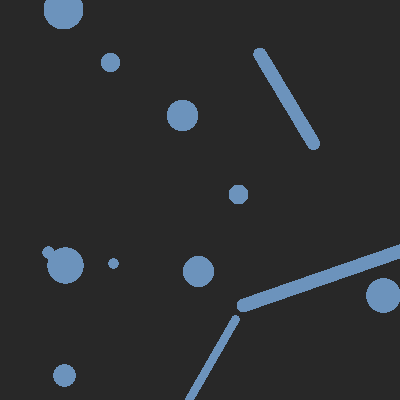
\includegraphics[width=\linewidth]{figures/generated-worlds/world_0.png}
        }
    \end{subfigure}
    \hspace*{\fill}
    \begin{subfigure}{\w}
        \makebox(\textwidth, \textwidth)[\textwidth]{
            
\includegraphics[width=\linewidth]{figures/generated-worlds/world_1.png}
        }
    \end{subfigure}
    \hspace*{\fill}
    \begin{subfigure}{\w}
        \makebox(\textwidth, \textwidth)[\textwidth]{
            
\includegraphics[width=\linewidth]{figures/generated-worlds/world_2.png}
        }
    \end{subfigure}

    \vspace{4mm}

    \begin{subfigure}{\w}
        \makebox(\textwidth, \textwidth)[\textwidth]{
            
\includegraphics[width=\linewidth]{figures/generated-worlds/world_3.png}
        }
    \end{subfigure}
    \hspace*{\fill}
    \begin{subfigure}{\w}
        \makebox(\textwidth, \textwidth)[\textwidth]{
            
\includegraphics[width=\linewidth]{figures/generated-worlds/world_4.png}
        }
    \end{subfigure}
    \hspace*{\fill}
    \begin{subfigure}{\w}
        \makebox(\textwidth, \textwidth)[\textwidth]{
            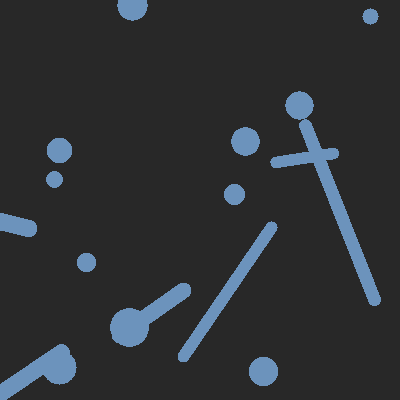
\includegraphics[width=\linewidth]{figures/generated-worlds/world_5.png}
        }
    \end{subfigure}
    \caption{Examples of generated environments.}
    \label{fig:generated-enviornments}
\end{figure}

\subsection{Training a Minimal Agent}
To ensure that the training framework works, a simple agent was trained. The agent is provided the same state as used in the Gradient behavior: Robot angle, the angle and distance to the closest obstacle, and the angle and length of the search gradient. The action space consists of 7 discrete actions, spanning from full left to forward to full right control commands. A single hidden layer of 64 nodes connects the input and output layers. The sigmoid activation function is used for all layers. \\

The agent was trained on 200 episodes, each consisting of 240 simulated seconds. The training progress is shown in \cref{fig:rl-minimal-training}.

\begin{figure}[H]
    \centering
    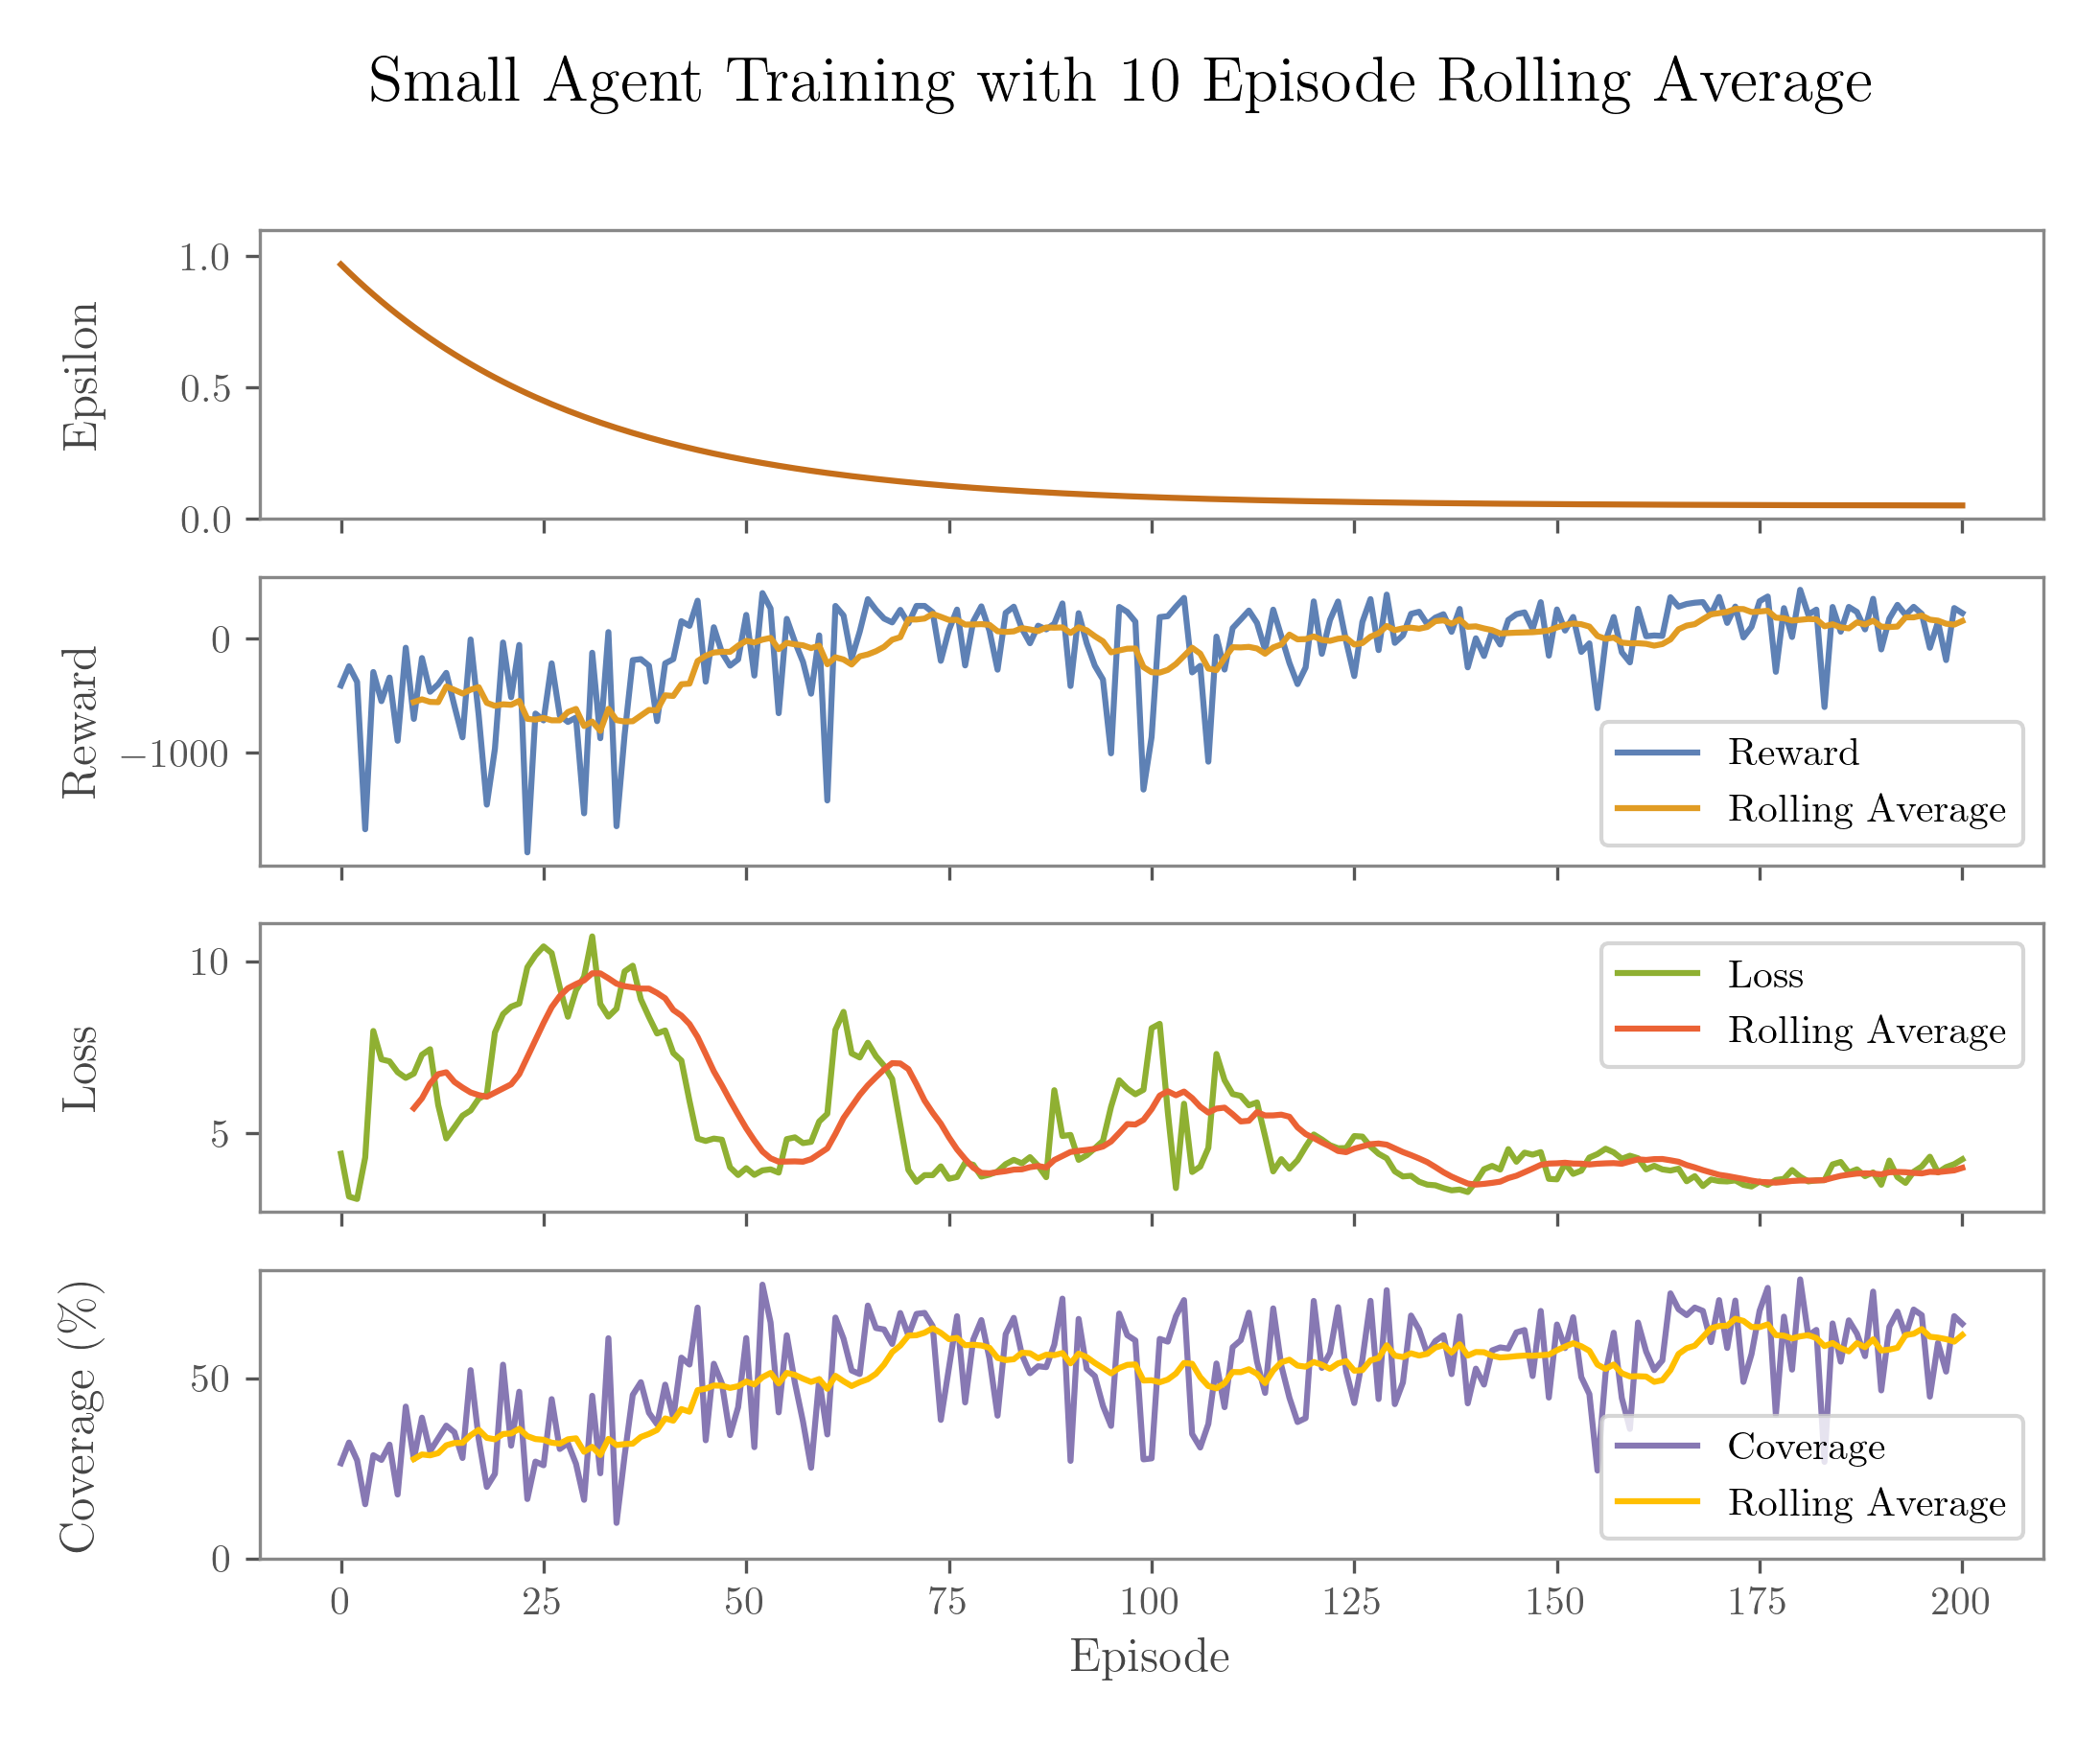
\includegraphics[width=0.95\textwidth]{figures/rl/small-search-agent-training.png}
    \caption{TODO}
    \label{fig:rl-minimal-training}
\end{figure}

As the agent is trained, the reward and coverage increases, indicating that the agent is learning to cover the map. The loss function also settles down eventually, which signifies that the model is predicting the reward function well. Running the behavior results in the path shown in \cref{fig:rl-minimal-path}.

\def\w{0.329\textwidth}
\begin{figure}[H]
    \centering
    \begin{subfigure}[b]{\w}
        \centering
        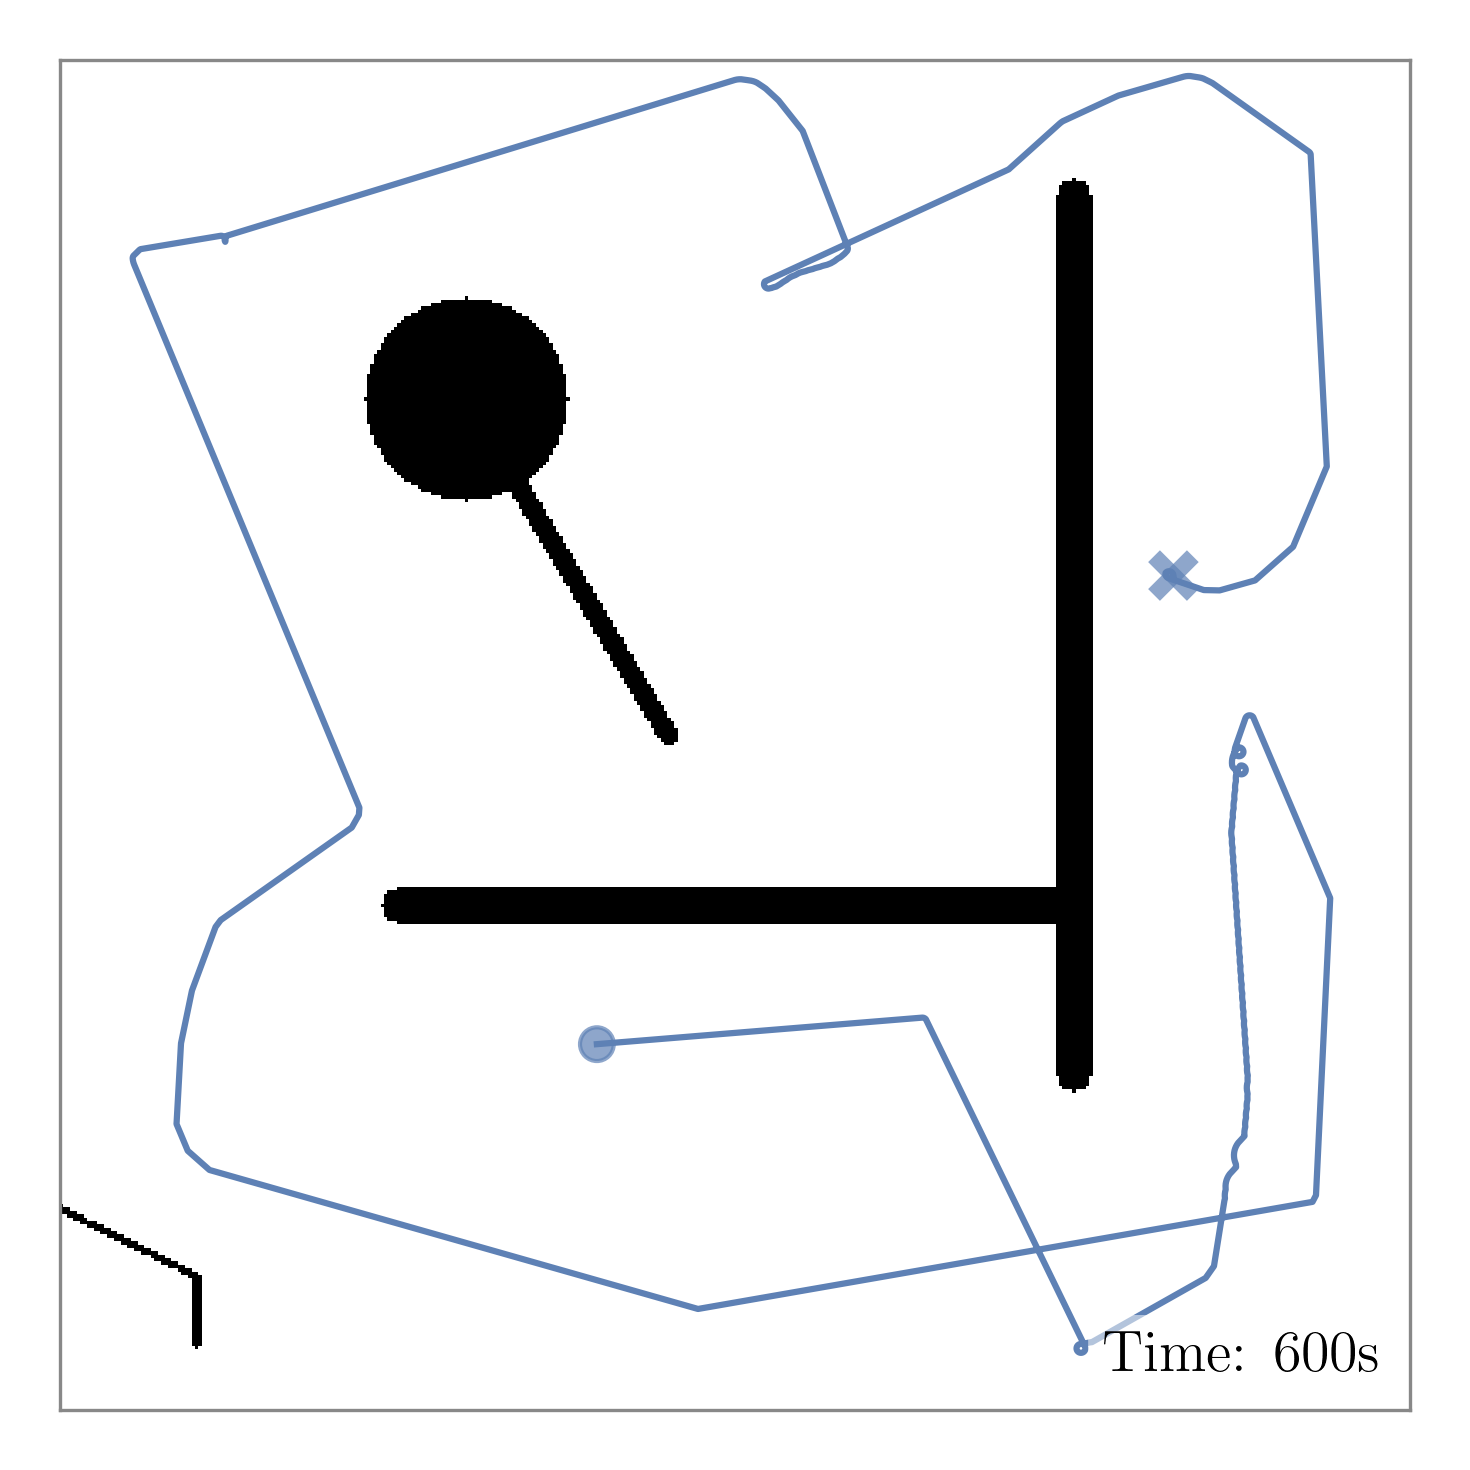
\includegraphics[width=\textwidth]{./figures/rl/small-agent-(after-600s).png}
    \end{subfigure}
    \begin{subfigure}[b]{\w}
        \centering
        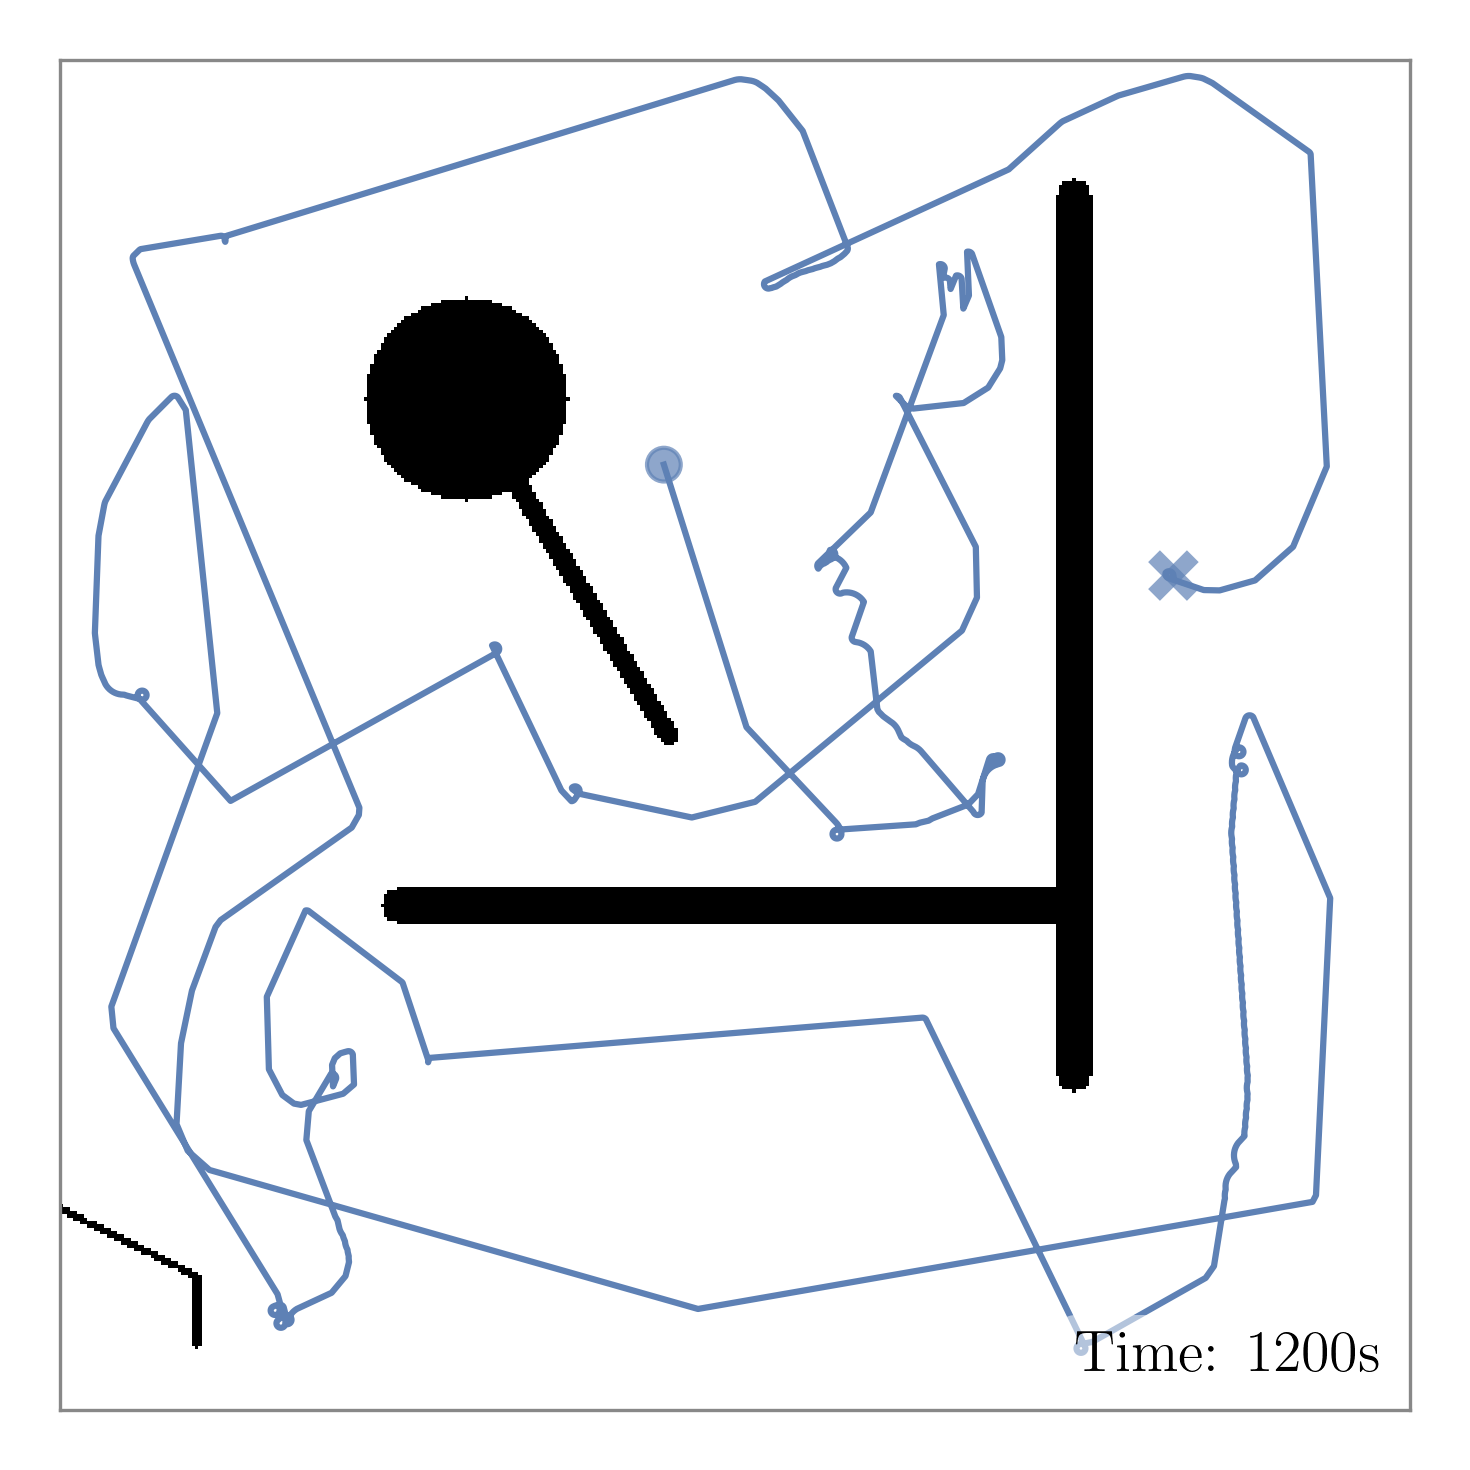
\includegraphics[width=\textwidth]{./figures/rl/small-agent-(after-1200s).png}
    \end{subfigure}
    \begin{subfigure}[b]{\w}
        \centering
        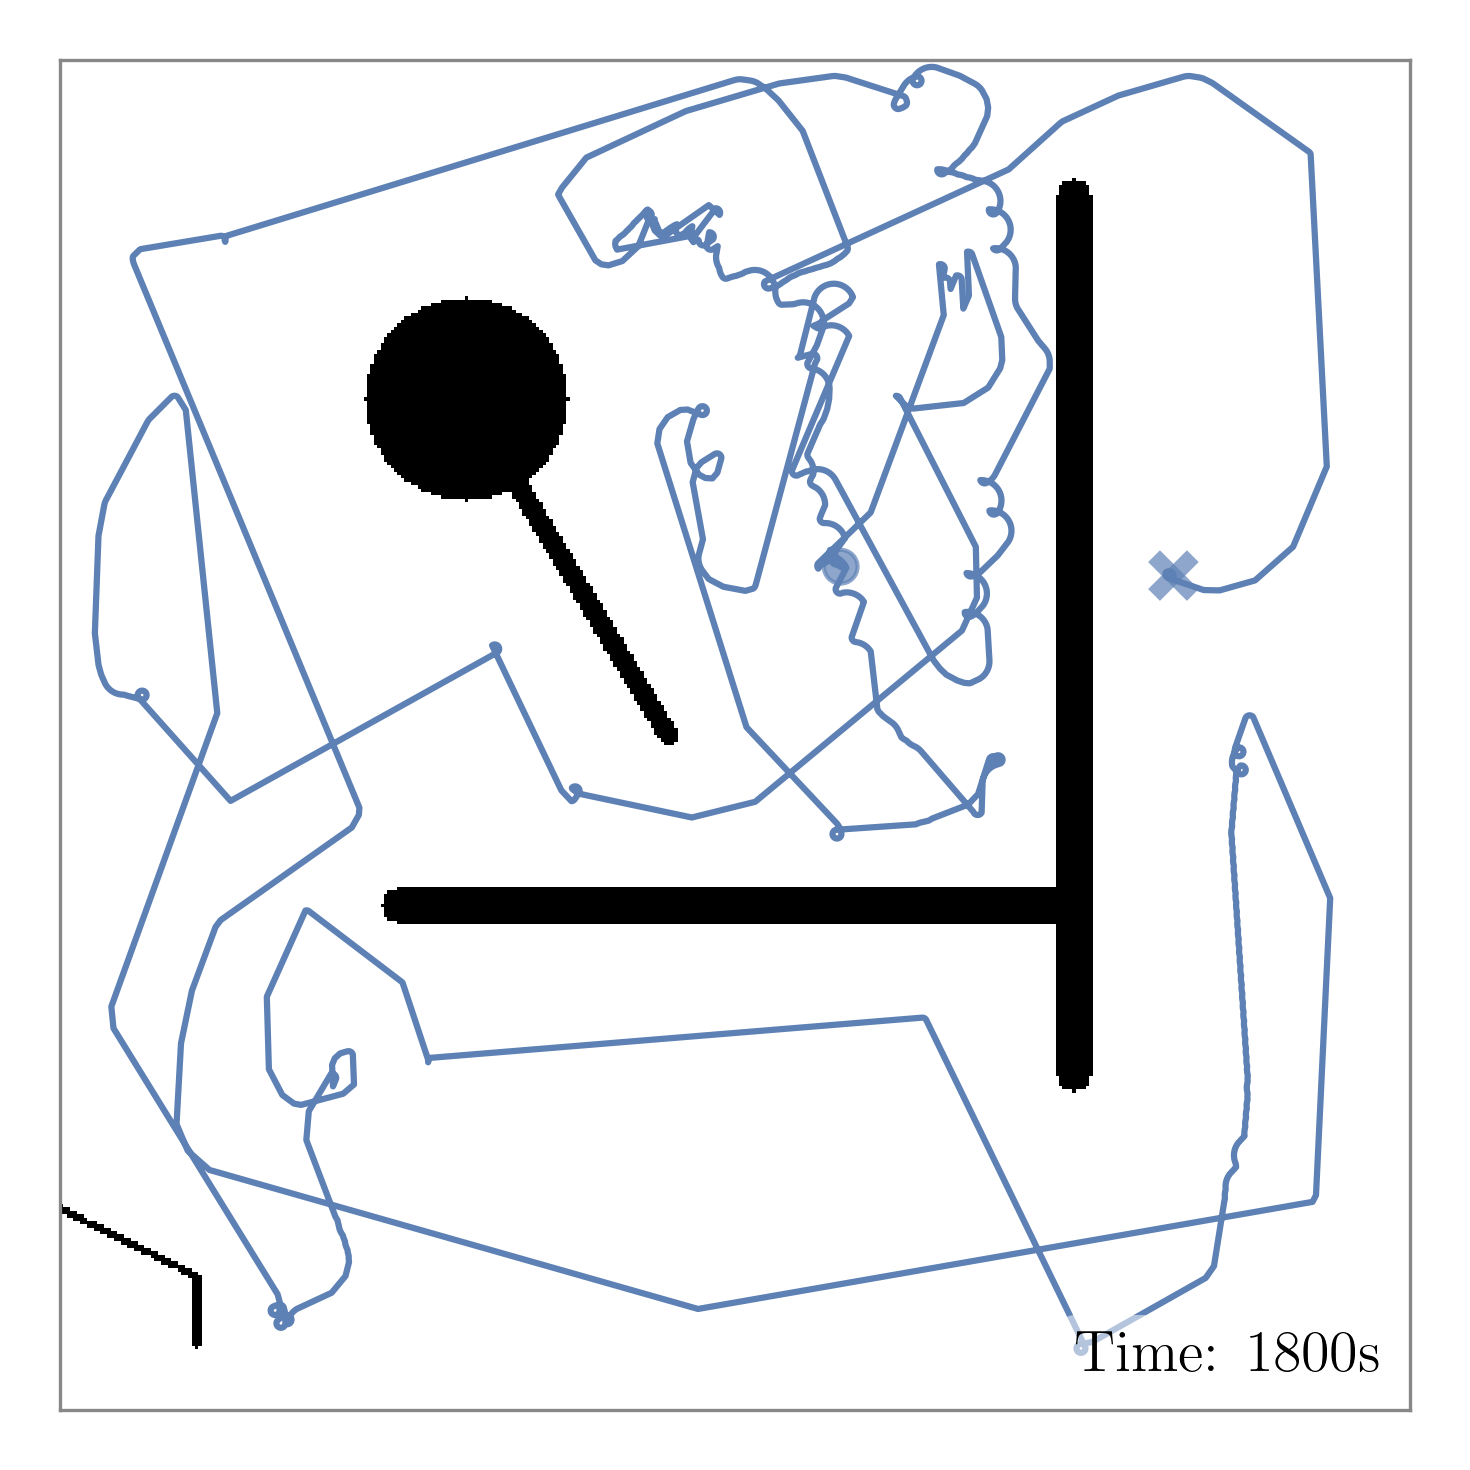
\includegraphics[width=\textwidth]{./figures/rl/small-agent-(after-1800s).png}
    \end{subfigure}
    \caption{TODO}
    \label{fig:rl-minimal-path}
\end{figure}

% TODO: Add flamegraph to appendix
\subsection{Training more Complex Agents}
While the successfully trained agent show that the framework works, training is very computationally expensive. The minimal agent took approximately 12 hours to train. This could be an issue with the trainer or simulator implementation, especially as the simulation steps take longer as training progresses. The trainer was run with a profiler to investigate this, which showed that approximately 75\% of the run time is spent within the \texttt{burn} framework. This leads to the conclusion that updating the model weights is most major factor in the training performance, and that faster hardware is needed to speed up training. \\

More complex agents are implemented in \texttt{botbrain} and training was attempted but never finished. An agent called \texttt{big-boy} was implemented to theoretically be aware of the robot swarm as a whole, and could therefore be trained to keep the swarm within communication range. The state input for the \texttt{big-boy} agent consists of the following fields:

\begin{itemize}
    \item Robot angle
    \item Average swarm angle
    \item 12 LiDAR rays
    \item Search gradient vector
    \item Vector to the closest robot
    \item Size of the swarm (robot count)
    \item Center of the swarm
    \item Spread of the swarm in $x$ and $y$ direction
\end{itemize}

This results in 25 input nodes. The action space consists of 9 actions in the same manner as the minimal agent. This model contains three hidden layers of 96, 64 and 32 nodes respectively. The larger network should make the agent capable of learning a more intricate behavior and make better sense of the increased input nodes. \\

In theory, the network inputs could be expanded even more to also include global knowledge of the map to increase performance. This could be implemented in the current framework, but was not, as training was deemed infeasible.
